\documentclass[UTF8]{ctexart}
\usepackage{geometry}
\usepackage{fancyhdr}
\usepackage{verbatim}
\usepackage{enumerate}
\usepackage{graphicx}
\usepackage{subfigure}
\usepackage[colorlinks,linkcolor=blue]{hyperref}
\graphicspath{{./Images/}}

\geometry{papersize={210mm,297mm}}
\geometry{left=2.5cm,right=2.5cm,top=2.5cm,bottom=2.5cm}

\setlength{\headheight}{13pt}

\title{SlopeCraft v3.6教程}
\author{TokiNoBug}
\date{\today}

\begin{comment}
\pagestyle{fancy}

\lhead{\author}
\chead{\title}
\rhead{\date}

\lfoot{}
\cfoot{\thepage}
\rfoot{}

\renewcommand{\headrulewidth}{0.4pt}
\renewcommand{\headwidth}{\textwidth}
\renewcommand{\footrulewidth}{0pt}

\end{comment}

\begin{document}
    \maketitle
    %%%%%%%%%%%%%%%%%%%%%%%
    % Page1
    %%%%%%%%%%%%%%%%%%%%%%%
    SlopeCraft v3.6是一个重大更新,整个程序都被重构了一遍,增加了许多硬核的功能,解决了不少棘手的麻烦:v3.6实现了期盼已久的有损压缩功能,可以把地图画总高度压缩到几乎任何值,彻底解决了地图画超出限高的问题;v3.6加入了“搭桥”功能,可以辅助玩家建造……
    
    除此以外,v3.6还修改了界面的操作逻辑。加之上一版教程还是v3.1,我认为有必要写个新的教程。

    这篇教程不是“傻瓜式”的,我只介绍必须介绍的,强调必须强调的。

    %%%%%%%%%%%%%%%%%%%%%%%
    % Page2
    %%%%%%%%%%%%%%%%%%%%%%%
    \pagebreak
    \section{v3.6更新内容简介}
    \paragraph{新内容}
    \textbf{SlopeCraftL3.dll}——SlopeCraft的内核开发成了通过接口类调用的\textbf{动态链接库},随应用程序一同发布,包含了立体、平板、纯文件地图画和墙面像素画的核心功能,理论上应该能被C++、Java、Python等语言调用(顶多再套一层接口),后来者可以\textbf{少造轮子}了!

    \paragraph{新功能}
    \begin{enumerate}
        \item 第61个基色:\textbf{发光地衣}——补上了v3.5.1的遗漏
        \item 智能有损压缩——\textbf{彻底解决超限高问题}
        \item 搭桥——\textbf{方便建造立体地图画}
        \item 防火/防末影人——用玻璃块包围\textbf{易燃方块}和\textbf{可被小黑偷走}的方块
        \item 导出为.NBT格式——\textbf{Litematica}和\textbf{原版结构方块}可以用,不知WorldEdit是否可用
        \item 方块增加了各种\textbf{下半砖}
        \item 自定义方块列表——更加自由,想要什么方块\textbf{自己加}
        \item 构建三维结构时预览地图画——\textbf{有损压缩可能会微调画面内容}
        \item 检查更新、反馈Bug——请认准GitHub仓库
        \item 更加完善的报错系统——\textbf{报错信息不是天书!}
        \item 启动时自动设置语言——默认简体中文,如果系统语言没有汉语,那就英文
        \item settings.json——启动时的配置文件
        \item 新的像素画类型:墙面像素画——不伦不类的东西,偏偏很多人想要这个功能
    \end{enumerate}
    \paragraph{修复Bug}
    \begin{enumerate}
        \item 修复了无法禁用部分颜色的Bug——重写了方块列表的逻辑 
    \end{enumerate}
    \paragraph{优化和其他更改}
    \begin{enumerate}        
        \item 优化了转化图片和搭桥的性能——感谢AbrasiveBoar902
        \item 删除了可去掉的“确认”按钮,节省操作
        \item 等待用户操作时进度条不再显示为繁忙状态,更符合操作习惯
    \end{enumerate}

    \pagebreak
    %%%%%%%%%%%%%%%%%%%%%%%
    % Page3
    %%%%%%%%%%%%%%%%%%%%%%%
    \section{初级教程}
    \subsection{导入图片}
    从上一个教程(v3.1)到v3.6,最大的变化其实还是多了个“设置”按钮,用来更好的处理原图中\textbf{透明像素}。
    
    点击\textbf{设置}按钮,可以看到如下子窗口:
%\begin{comment}
    \begin{center}
        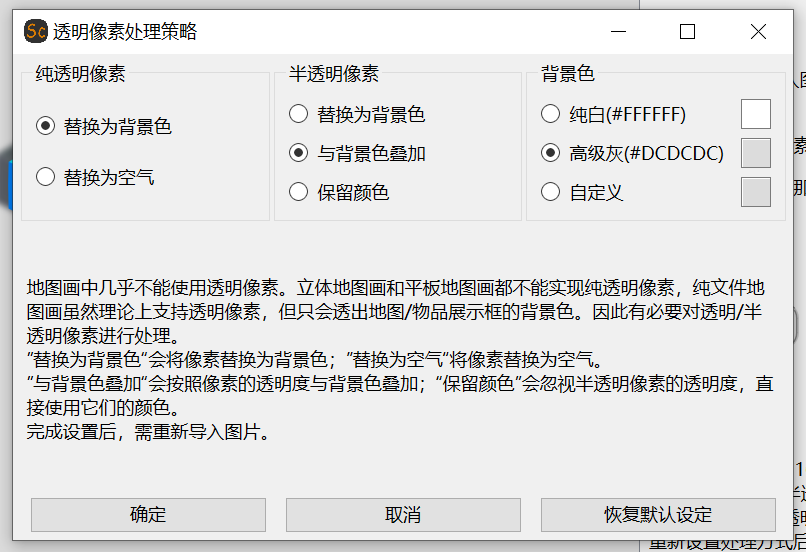
\includegraphics[width=15cm]{Img1_TPS.png}
    \end{center}
%\end{comment}

    \textbf{请注意:如果你要按照自定义的策略导入含全透明/半透明像素的图片,务必先设置透明像素处理策略,后导入图片!否则图片只会按照默认的处理策略处理!如果已经导入了图片才重新设置处理策略,请重新导入图片!}

    \subsection{设置地图画类型}
    地图画类型中多了一项墙面像素画。除此以外没有改动。只需要按说明设置地图画类型及版本,然后直接跳转到下一页即可。

    设置方块列表页面补加了第61个基色:发光苔藓。
    请注意方块列表的逻辑:灰色的按钮/选择框代表锁定、不可更改的,如基色0(透明)必须启用。SlopeCraft要求每种基色必须有对应的方块,哪怕这种基色本身被禁用,因此如果某个基色只有一种方块可选,那个唯一的单选框也是锁定的。另外,有些方块是墙面像素画不能使用的,如铁质压力板、发光苔藓等。这时限制颜色数量的不是基色/地图色本身的性质,而是你所选的方块。

    \subsection{调整颜色}
    调整颜色界面也没有值得一提的改变,只需要选好算法,点击\textbf{转化},然后选择你想要的导出方式。这里以Lancet\_Corgi画的图为例,这也是常用的测试用图之一(感谢刀妈\~)
\begin{comment}
    \begin{figure}[htbp]
        \centering
        \subfigure[a]{
            \begin{minipage}{6cm}
                \centering
                
\includegraphics[width=5cm]{Img3_Raw.png}
                \caption{原图}
            \end{minipage}
        }
        \subfigure[b]{
            \begin{minipage}{6cm}
                \centering
                
\includegraphics[width=5cm]{Img4_Converted.png}
                \caption{转化后}
            \end{minipage}
        }
        \caption{导入原图并按RGB+算法(无抖动)转化}
    \end{figure}
\end{comment}
    \subsection{导出三维结构}
    压缩高度一栏增加了\textbf{智能有损压缩};增加了\textbf{搭桥}选项;增加了\textbf{防火}和\textbf{防末影人}选项。
\begin{comment}
        \begin{center}
        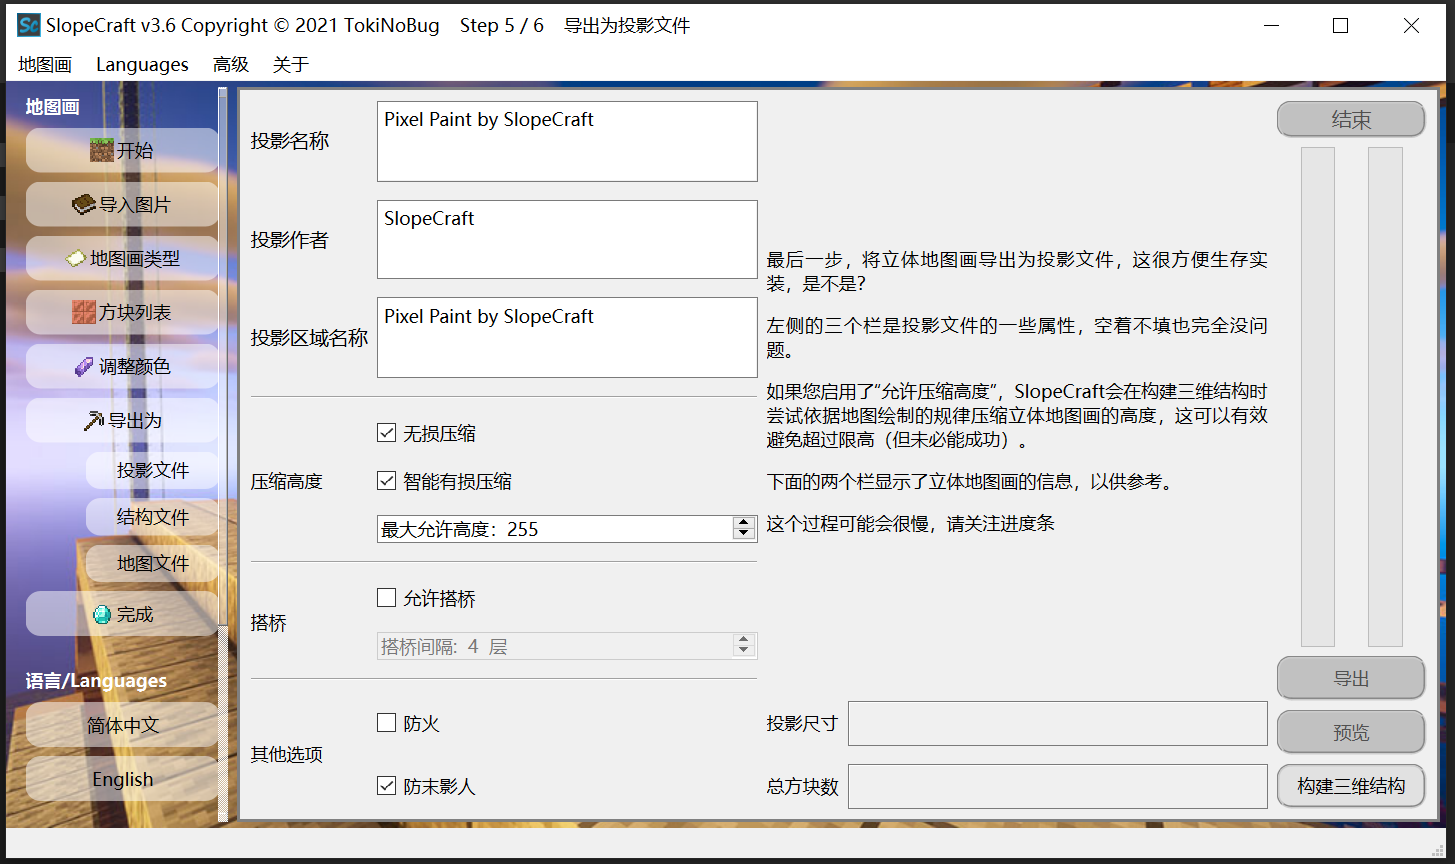
\includegraphics[width=15cm]{Img2_Export3D.png}
    \end{center}
\end{comment}

    \subsubsection{压缩}
    简单来说,无损压缩是在\textbf{严格保证每个像素颜色不变}的前提下,压缩地图画总高度,但它约束较大,未必如愿。
    有损压缩则\textbf{微调个别像素的颜色},压缩地图画总高度,使其小于等于用户指定的最大允许高度。有损压缩使用的是遗传算法,属于群体人工智能,是目前SlopeCraft中技术含量最高的模块。最大允许高度不要低于14,否则立体地图画很可能压缩失败。

    有损压缩和无损压缩可以搭配使用,也可以分别独立使用。但一般来说,如果启用了有损压缩,没道理不启用无损压缩。因为纯有损压缩对画质的损伤会比较大,无损压缩能很大程度上减轻画质损伤。
    
    平板地图画和墙面像素画可以勾选这两个选项,但\textbf{不会发挥任何作用}。

    更多有关地图画的压缩,可阅读\href{https://github.com/ToKiNoBug/SlopeCraftTutorial/blob/main/BasicPrinciple/Principle%20of%20map%20pixel%20arts.md}{地图画原理}。

    \subsubsection{搭桥}
    立体地图画的每个水平截面上都有很多分散的方块,极不方便建造,倘若能用多条通路连接这些分散的方块,无疑能让建造更加容易。搭桥就是在一个水平面内用玻璃方块连接所有方块,形成通路从而辅助玩家建造的过程。
    
    毫无疑问,搭桥会消耗额外的玻璃,因此不推荐在立体地图画的每一层都执行搭桥。默认每间隔4层搭一次桥,你也可以修改这个间隔。间隔过大,辅助搭桥的效果会减弱;间隔过小,浪费玻璃。




\end{document}